
We describe  \sys's architecture and basic operation in Section~\ref{ssec:overview}.
We then discuss in-memory compaction policies  in  Section~\ref{ssec:policies}
and implementation details and thread synchronization in Section~\ref{ssec:impl-details}.
Section~\ref{ssec:offheap} discusses the   index layout in off-heap allocation.


\subsection{Overview} \label{ssec:overview}


\sys\ introduces a \emph{compacting} memory store to the LSM store design framework. In contrast to the traditional memory store, 
which maintains RAM-resident data in a single monolithic data structure, \sys\ manages data as a \emph{pipeline} of 
\emph{segments} ordered by creation time. Each segment contains an index over a collection of data cells.
At all times, the most recent segment, called \emph{active}, is mutable;
it absorbs put operations. The rest of the segments are immutable.  
%
In addition to searching data in the disk store, get and scan operations traverse all memory segments,  similarly to a traditional LSM store read from multiple files. 
\eshcar{ explain that we can in some cases skip some of the segments...}
  
Figure~\ref{fig:accordion} illustrates the \sys\ architecture. It is parameterized by two values:
\begin{itemize}
\item  $A$ --  fraction of the memory store allocated to the active segment; and 
\item $S$ --  upper bound on the number of immutable segments in the pipeline. 
\end{itemize}

\begin{figure}[tb]
\center
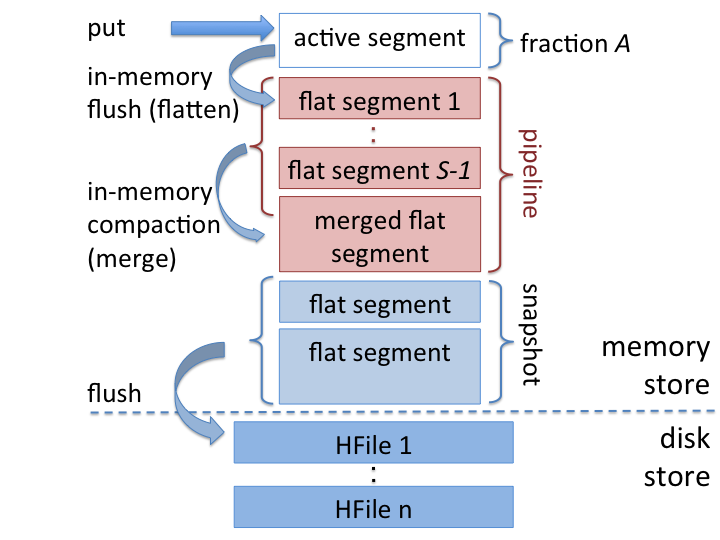
\includegraphics[width=\columnwidth]{accordion-arch} 
\caption{\sys's compacting memory store architecture adds a pipeline of flat segments between the active segment and the snapshot. 
The memory store includes a small dynamic active segment 
and a pipeline of flat segments. A disk flush creates a snapshot of the pipeline for writing to disk.}
\label{fig:accordion}
\end{figure}

\noindent
As our experiments show (Section~\ref{sec:eval}), the most effective parameter values are quite small, 
e.g., $0.02 \leq A \leq 0.05$, and $2 \leq S \leq 5$.

Once the active segment grows to its size bound (a fraction $A$ of the memory store's size bound), an \emph{in-memory flush} is invoked.
The in-memory flush makes the active segment immutable and creates a new active segment to replace it. 

In case there is available space in the pipeline (the number of pipeline segments is smaller than $S$), the replaced active segment is simply \emph{flattened}  and 
added to the pipeline. Flattening a segment involves replacing the dynamic segment index (e.g., skiplist) by a compact ordered array suitable for immutable data, as shown in Figure~\ref{fig:flattening}.
The indexed data cells are unaffected by the index flattening.

The flat index is more compact than a skiplist, and so reduces the MemStore's memory footprint, which delays  disk flushes, positively affecting both read latency  (by increasing the MemStore's hit rate) and write volume.
It is also cache- and GC-friendly,  and supports fast lookup via binary search.   
In managed environments, it can be allocated in off-heap (unmanaged) memory, which can improve performance predictability as  discussed in Section~\ref{ssec:offheap} below.

\begin{figure*}[t]
\center
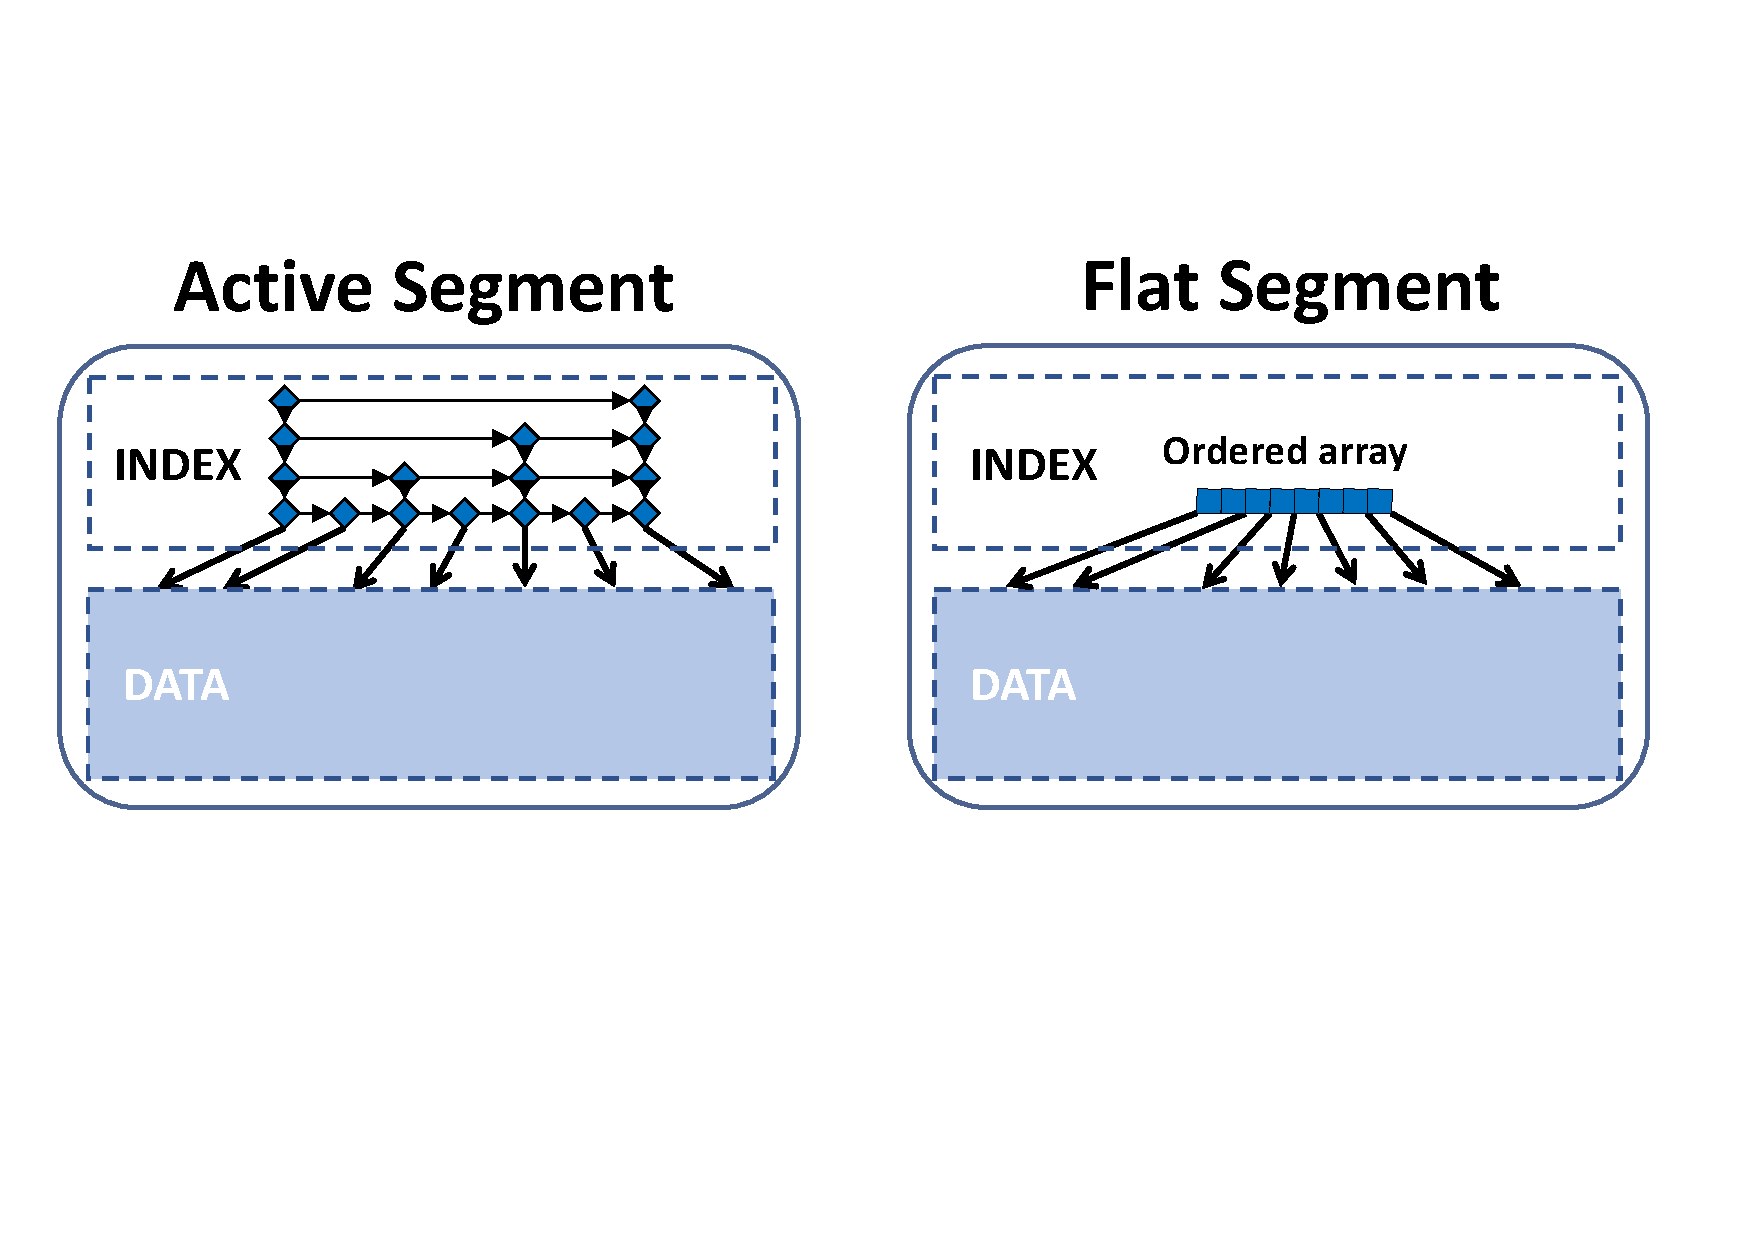
\includegraphics[width=\columnwidth]{flattening.pdf} 
\caption{Flattening converts an active segment with a skiplist index into a flat segment indexed by an ordered array. 
The data remains untouched. }
\label{fig:flattening}
\end{figure*}

Once the number of immutable segments exceeds $S$, the segments in the pipeline are processed to reduce their number.
At a minimum, an \emph{in-memory merge} replaces the indices of multiple segments by a single index covering data that was 
indexed by all original segments,  
\inred{as shown in Figure~\ref{fig:flattening}(c)}. 
This is a lightweight process that results in a single segment but does not eliminate redundant data versions.
For example, if a cell with the same row key and column key is stored in two different segments in the pipeline (with two different timestamps) then after the merge both cells will appear consecutively in the merged segment. 

Optionally, an \emph{in-memory compaction} can further perform \emph{redundant data elimination} by
creating a single flat index with no redundancies and disposing redundant data cells,  
\inred{as shown in Figure~\ref{fig:flattening}(d)}.  
In the example above only the more recent cell will appear in the compacted segment.
In case the memory store manages its cell data storage internally (via MSLAB), the surviving cells are relocated
to a new chunk (to avoid internal chunk fragmentation). Otherwise, the redundant cells are simply de-referenced, allowing the garbage-collector to reclaim them.    

The choice whether to eliminate redundant data (i.e., perform compaction) or not (perform only merge) is guided by the policies described in Section~\ref{ssec:policies} below.

Flushes to disk work the same way as in a standard LSM store: A disk flush first shifts all pipeline segments to the snapshot, which is not part of the pipeline, while the pipeline is emptied so that
it may absorb new flat segments. 
A background flush process merges all snapshot segments while eliminating  redundancies, and streams the result to a new file. 
After the file is written, the snapshot segments are freed. 

In case the disk flush process empties the pipeline while an in-memory compaction  is attempting to merge some segments, the latter aborts.  This behavior is valid since in-memory compactions are an optimization.

\subsection{Compaction Policies} \label{ssec:policies}

Redundant data elimination induces a tradeoff. On the one hand,
merging only search indices without removing redundancies is a lighter-weight process.  
Moreover, this approach is friendly to the managed memory system because the entire segment is freed at once, whereas 
removing (redundant) cells from existing segments burdens the memory management system (in particular, the garbage collector) by
constantly releasing small objects. On the other hand, by forgoing redundant data elimination we continue to 
consume memory for overwritten data; this is significant in production-like heavy-tailed distributions where some keys are frequently overwritten.
Removing these redundancies further delays disk flushes, which both improves read latency  (thanks to more 
queries being satisfied from memory) and reduces the write volume.

Our HBase 2.0 implementation includes the two extreme memory compaction policies:
\begin{description}
\item[\basic] (low-overhead) never performs redundant data elimination. Rather, 
once a segment becomes immutable, flattens its index, and once the pipeline size exceeds $S$, merges all segment indices into one.   
\item[\eager] (high-overhead, high-reward under self-similar workloads) immediately merges a segment that becomes immutable 
with the current  (single) pipeline segment, while eliminating redundant data.
%Once a segment becomes immutable, merge its index and data with the current (single) pipeline segment.
% In addition to \basic\/ mechanisms, eliminate data redundancies across pipeline segments.
\end{description}

Our experiments (reported in the next section) show that the \eager\ policy is typically too aggressive, in particular when $A$ is small,
and the benefits from reducing the memory footprint are offset by the increased management (and in particular, garbage collection) overhead.
We therefore present in this paper a third policy:
\begin{description}
\item[\adp] (the best of all worlds) a heuristic that chooses 
whether to eliminate redundant data  (as in \eager) or not (as in \basic) based on the level of redundancy in the data 
and the perceived cost-effectiveness of compaction. \adp\ works at the level of a single LSM store, i.e., triggers 
redundancy elimination only for those stores where positive impact is expected. 
\end{description}

\adp\ uses two parameters to determine whether to perform data redundancy elimination:
\begin{enumerate}
\item
%The first is 
A throttling parameter $t$  grows with the amount of data that can benefit from redundancy elimination. 
Initially, $t=0.5$; it then grows exponentially by $2\%$ with the number of in-memory flushes, and is reset back to 
the default value (namely $0.5$) upon disk flush. Thus, $t$ is bigger when there is more data in the MemStore.
\item
The \emph{uniqueness} parameter, $u$, estimates the ratio of unique keys in the memory store based on the 
fraction of unique keys encountered during the previous merge of segment indices. 
\end{enumerate}

Note that the accuracy of $u$ at a given point in time depends on the number of merges that occurred since the last disk flush
or data-merge.
Initially, $u$ is zero, and so the first in-memory compaction does not employ data-merge.
Then, the estimate is based on the $S$ merged components, which at the time for the second in-memory compaction
is roughly one half of the relevant data, since the pipeline holds $S-1$ unmerged components. 
Over time, $u$ becomes more accurate while $t$ grows. 

\adp\/ triggers redundancy elimination with probability $t$ if the fraction of redundant keys $1-u$ exceeds a parameter 
threshold $R$. The rationale for doing so is that prediction based on $u$ becomes more accurate with time, whence 
compactions become more important because the component is bigger and more space can be saved.


\eshcar{ add description of WAL truncation}

\subsection{Concurrency} \label{ssec:impl-details}

A compacting memstore is comprised of an active segment and a double-ended queue (pipeline) of inactive segments. 
The pipeline is accessed by read APIs (get and scan), as well as by background disk flushes and in-memory compactions. 
The latter two modify the pipeline by adding, removing, or replacing segments. These modifications happen infrequently. 

The pipeline's readers and writers coordinate through a lightweight copy-on-write, as follows. 
The pipeline object is versioned, and updates increase the version.

Reads access the segments lock-free, through the version obtained at the beginning of the operation. 
If an in-memory flush is scheduled in the middle of a read, the active segment may migrate into the pipeline. 
Likewise, if a disk flush is scheduled in the middle of a read, a segment may migrate from the pipeline to the pre-flush snapshot buffer. 
The correctness of reads  is guaranteed by first taking the reference of the active segment then the pipeline segments and finally the snapshot segments. This way, a segment may be encountered twice but no data is 
lost. The scan algorithm filters out the duplicates. 

 Each modification takes the following steps: 
(1) promotes the version number;
(2) clones the pipeline, which is a small set of pointers, 
(3) performs the update on the cloned version, and
(4) uses a compare-and-swap (CAS) operation to
atomically swap the global reference to the new pipeline clone, provided that its  version did not change since (1).
Note
that cloning is inexpensive -- only the segment references are copied since the segments themselves are immutable. 
\remove{
In-memory compaction is a read-modify-write operation, which swaps one or more segments in the pipeline 
with a new segment built from their data. This operation's atomicity is guaranteed by a compare-and-swap (CAS) operation
that flips the pipeline version only if the latter did not change since the compaction started.  
}
For example, in-memory
compaction fails if a disk flush concurrently removes some segments from the pipeline.
% (Section~\ref{ssec:overview}). 


\subsection{Off-Heap  Allocation} \label{ssec:offheap}
As explained above, prior to \sys, HBase allocated its MemStore indicies on-heap, using a standard Java skiplist for the active buffer and the snapshot. \sys\ continues to use the same data structure -- skiplist -- for the active segment, but adopts arrays for the flat segments and snapshot. 
Each entry in an active or flat segment's index holds a reference to a cell object, which holds a reference to a buffer holding a key-value pair (as pojo or in MSLAB),
as illustrated in Figure~\ref{fig:on-heap}(a). 
HBase MSLAB chunks may be allocated off-heap. 

\begin{figure*}[tbh]
\center
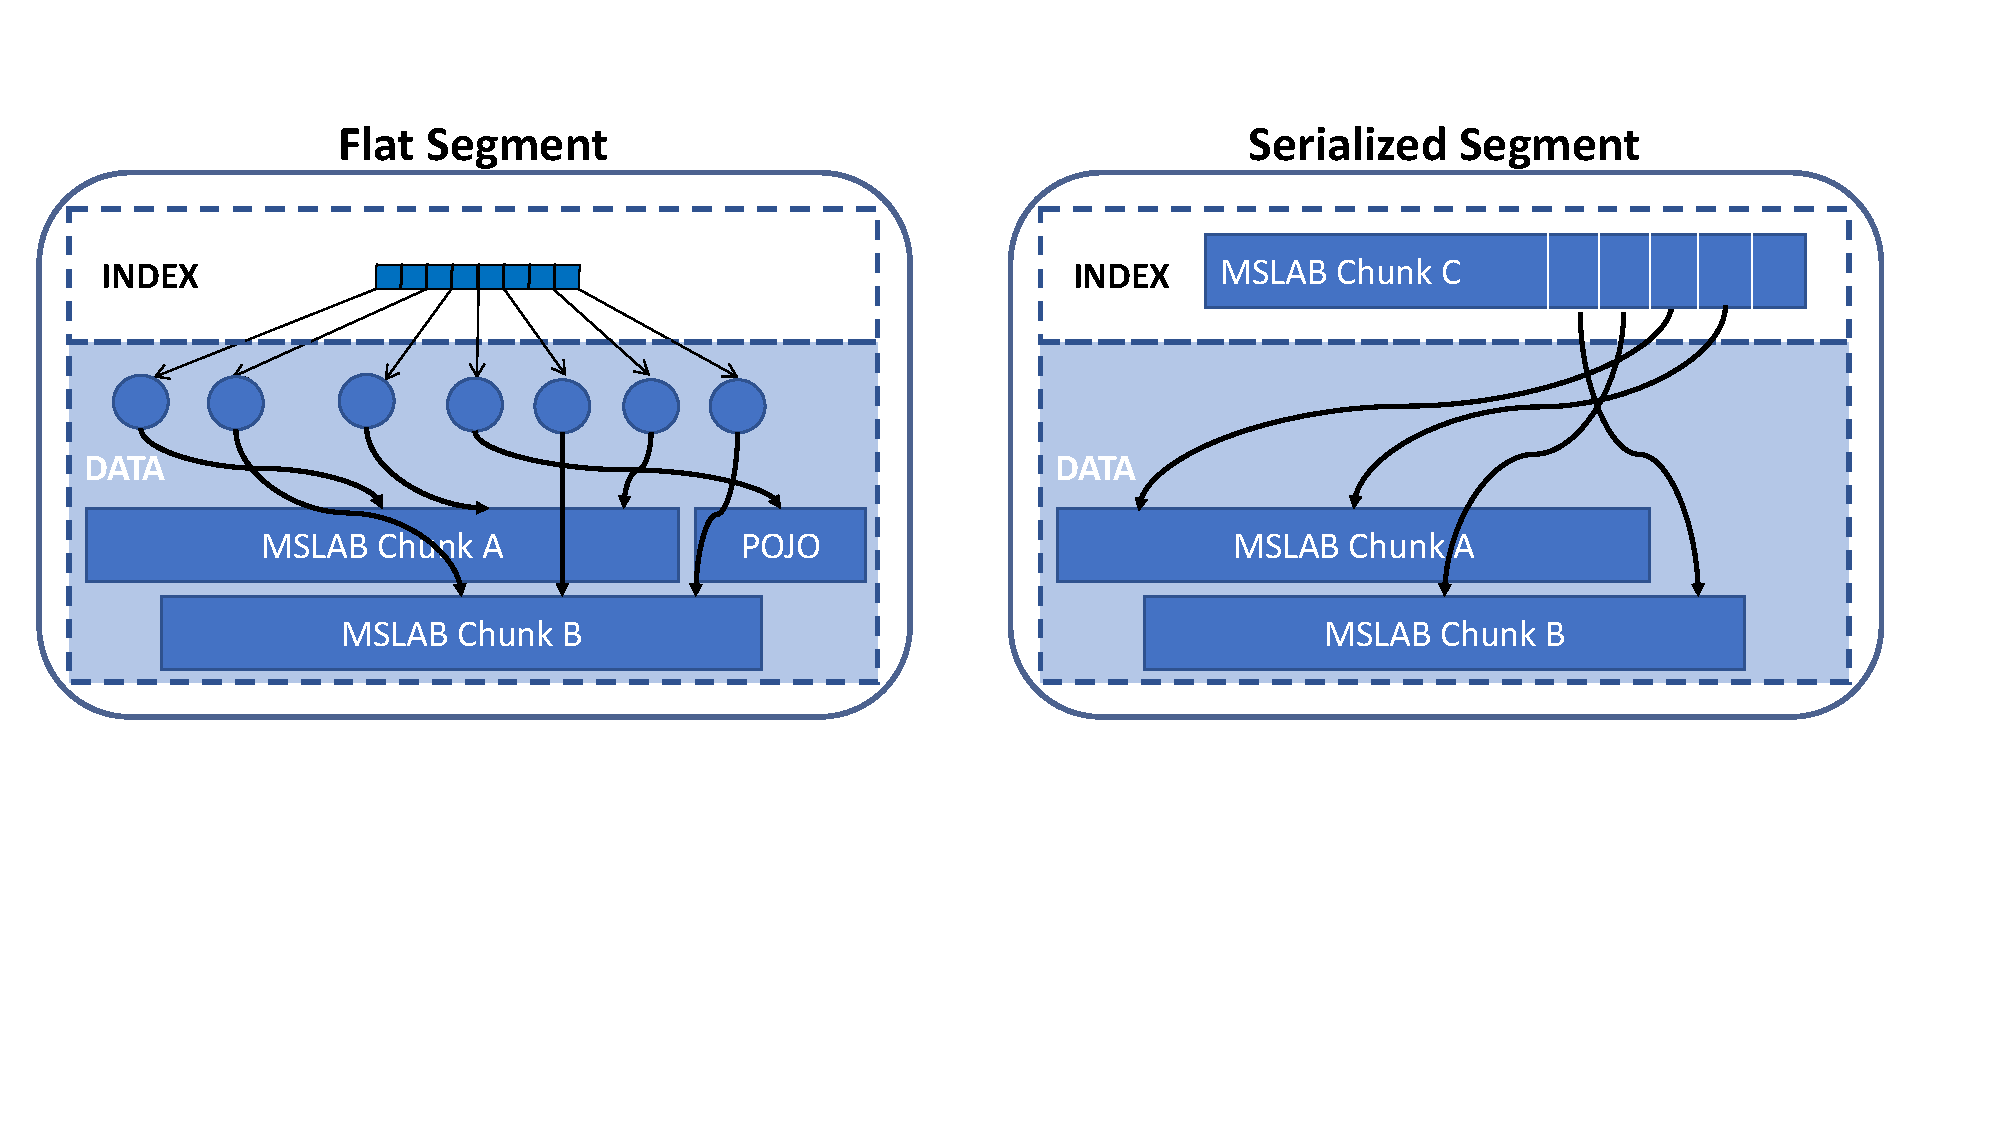
\includegraphics[width=0.9\columnwidth]{serializing.pdf} 
\caption{The difference between the flat segment and the serialized segment. The ordered array of the cell objects cannot be directly serialized and streamed into an off-heap chunk. The transformation shrinks the cell object into just 20 bits, and writes on the index chunk.}
\label{fig:on-heap}
\end{figure*}
%\begin{figure}[tbh]
%\center
%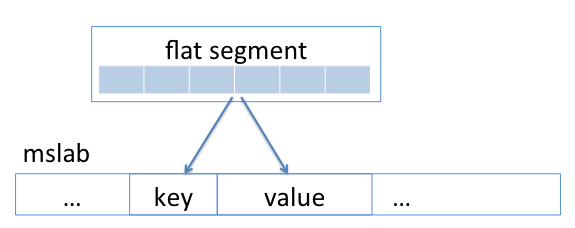
\includegraphics[width=0.75\columnwidth]{off-heap} 
%\caption{Off-heap allocated flat segment referencing data that resides in mslabs.}
%\label{fig:off-heap}
%\end{figure}

\sys's \emph{serialized} version takes this approach one step further, and allocates the flat segment index
using MSLAB as well as the data. 
A serialized segment has its index and data allocated via the same MSLAB object, but on different chunks. 
Each MSLAB may reside either on- or off-heap.

Serialized segments forgo the intermediate cell
objects, and have array entries point directly to the the chunks holding keys and values, as illustrated in 
Figure~\ref{fig:on-heap}(b).  
Removing the cell objects yields
a substantial space reduction, especially when data items are small, and eliminates the intermediate level of indirection.

 Offloading  data from the Java heap
has been shown to be effective for read traffic~\cite{alibabahbase}. However, it necessitates recreating temporary
cell objects to support HBase's internal scan APIs. Nevertheless, such temporary objects consume  a small amount of space on-demand, 
and these objects are  deallocated rapidly, making them easier for the GC process to handle.



